\chapter{Introduction} \label{chap: Introduction}

The standard model (SM) gathers the entire understanding about fundamental particles and their interactions. Although the model has successfully explained various physical phenomena observed experimentally, there are still multiple unanswered questions concerning particle physics. For example, experiments \cite{Detectores} have shown that accelerator and reactor, solar, and atmospheric neutrinos have mass by proving the existence of neutrino oscillations. The fact that there are neutrino oscillations contradicts the SM, because this model predicts that neutrinos are massless. Some specific experiments for each neutrino category are: Super-Kamiokande \cite{Super-Kamiokande} for solar and atmospheric neutrino oscillations, KamLAND \cite{KamLAND} for reactor neutrinos, and K2K \cite{K2K} for accelerator neutrino oscillations \cite{Experimentos}. An additional open question about neutrinos is the fact that only neutrinos with left helicity have been observed. Helicity is defined as the projection of the particle's momentum vector over its spin direction. Therefore, only neutrinos with spin anti-parallel to its linear momentum have been detected.

In order to provide neutrinos with mass, several theories that extend the predictions of the SM have been proposed. One of the most known models is the "see-saw" or balance mechanism \cite{See-saw}. This mechanism postulates the existence of a yet undetected particle called the heavy neutrino. This heavy neutrino would have a mass inversely proportional to the one of the neutrino, thus making the mass of the heavy neutrino considerably large. Also, this neutrino would have a right helicity therefore restoring the right-left symmetry in the standard model. Other models that try to provide mass to the neutrinos by extending the SM postulate the conservation of the $(B-L)$ number, where $B$ is the baryon number and $L$ is the lepton number. Unlike these models, the see-saw mechanism proposes a breaking in the $(B-L)$ symmetry with consequences discussed in the next paragraph.

The see-saw mechanism includes three sub-models that provide mass to neutrinos. These three models come from the fact that is necessary to take into account the effects of breaking the $(B-L)$ symmetry. This effects can be parametrized using a Weinberg operator of the form $\lambda_{ll^{\prime}}L_{l}L_{l^{\prime}}\Phi\Phi/\Lambda$ where $\Phi = (\phi^{+}, \phi^{0})^{\intercal}$ is the doublet associated with the SM Higgs Boson and $L_{l} = (\nu_{l},l)_{L}^{\intercal}$ the representation of a doublet field associated with the lepton number +1 \cite{See-saw}. Since there are only three ways in which this Weinberg operator can be obtained at tree-level, there are also three types of the see-saw mechanism. In the type I see-saw mechanism the product between $L_{l}$ and $\Phi$ results in a fermionic singlet state . In the type II see-saw mechanism, the product between $L_{l}$ and $L_{l^{\prime}}$ forms a scalar triplet. Finally, the product between $L_{l}$ and $\Phi$ in the type III sub-model results in a fermionic triplet state. The state formed by the products described in each see-saw model would correspond to the definition of heavy neutrino in each sub-model. Taking into account the elements described above regarding the see-saw mechanism, if heavy neutrinos are observed, the left and right symmetry in the SM would be restored and the mechanism by which the neutrinos acquire mass would be explained.

Heavy neutrinos searches have been conducted in multiples experiments, but none has been able to prove that heavy neutrinos exist. Examples of these experiments can be found in collaborations such as LEP \cite{LEP}, CMS and ATLAS \cite{CMS ATLAS}. In order to understand heavy neutrino searches it is necessary to define the concept of jet. A jet at phenomenological level is defined as a quark or a gluon. In high energies experimental physics, a jet is defined as a collection of particles resulting from the fragmentation of quarks or gluons. Searches at CMS and ATLAS have focused in final states with associated leptons and jets. Figure \ref{fig: W} shows a Feynman diagram of the production of a heavy neutrino mediated by a W boson with left or right helicity. The final state for this process has two leptons ($\mu$, $e$, or $\tau$) and two jets.

\begin{figure}[H]
\centering
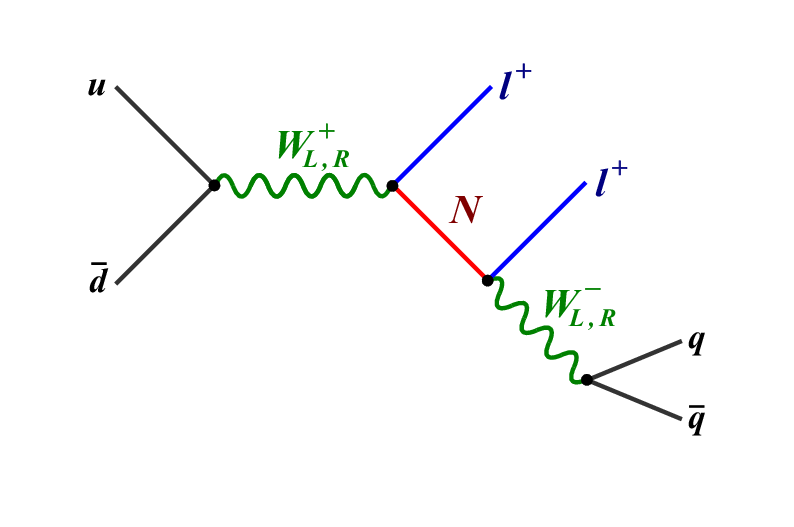
\includegraphics[width=\linewidth]{Figures/Feynman_W.png}
\caption{Feynman diagram of heavy neutrino production. (Taken from \cite{CMS ATLAS})}
\label{fig: W}
\end{figure}

The main objective of this monograph is to perform a phenomenological study about the feasibility of conducting an experimental analysis for the detection of heavy neutrinos in the Large Hadron Collider (LHC) using a technique known as vector boson fusion (VBF). This technique has been recently used in the LHC \cite{VBF Search} in searches for new physics. In high energy physics, the bosons $W^{\pm}$, $Z^{0}$ and $\gamma$ are known as vector bosons. The process of vector boson fusion occurs through an electroweak interaction of associated quarks with the LHC proton beams. The VBF topology consists in requiring two highly energetic jets in the longitundinal region of the detector and in opposite hemispheres thereof. It has been shown that by requiring this type of event, the noise level (background) is reduced considerably in regions of difficult study in searches of new physics.
%In the analysis, the production of heavy neutrinos is considered through the decay of a high mass hypothetical resonance known as $Z^{'}$ (shown in the Feynman diagram of Figure \ref{fig: VBF}). This high mass resonance comes from the vector boson fusion process.

%\begin{figure}[H]
%\centering
%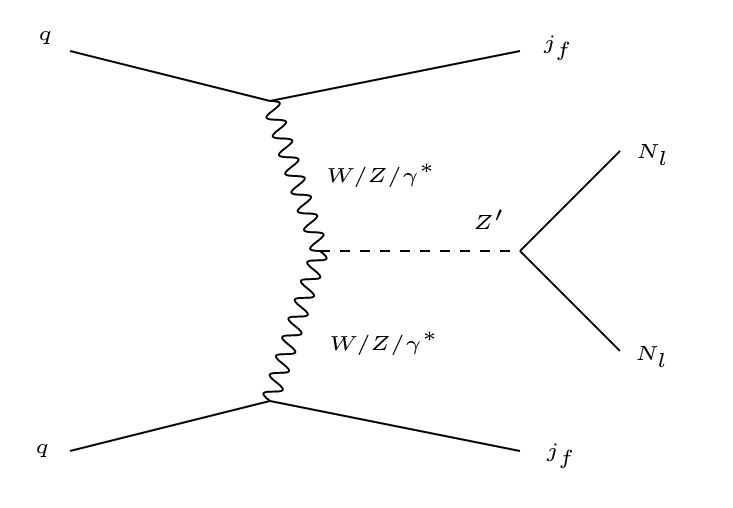
\includegraphics[scale = 0.65]{Figures/Feynman_VBF.JPG}
%\caption{Feynman diagram of VBF process.}
%\label{fig: VBF}
%\end{figure}

%The production of the heavy neutrino consists in the interaction of two quarks associated to the protons colliding in the beam. The protons emit vector bosons that produce a heavy resonance when they fuse. The heavy resonance decays afterwards producing the heavy neutrinos ($N_{l}$): $pp \rightarrow jj Z^{'} \rightarrow jj N_{l}N_{l}$.




In order to conduct the analysis, it is important to simulate signal and background processes and to perform a detailed physical study of the variables that allow to distinguish signal for experimental noise. It is necessary to use a cuantitative estimator commonly known as figure of merit to determine optimal cuts in the mentioned variables. The latter with the objective of reducing the amount of experimental noise by finding the optimal cuts in the relevant variables. For this particular analysis, the significance formula that will be used is the one shown in Equation \ref{eq: significance}, where $S$ is the significance, $N(s)$ is the number of signal events, and $N(B)$ is the number of background events.

\begin{equation} \label{eq: significance}
    S = \frac{N(s)}{\sqrt{N(s) + N(B)}}
\end{equation}

Furthermore, it is important to establish the expected experimental sensitivity using maximum likelihood limits or the calculation of the final significance for different hypothetical signal points. The procedure described would allow to conclude whether a study for the detection of heavy neutrinos at the LHC is feasible or not.
